\chapter{Organización funcional de la célula eucariota}\label{ch:b1:eukaryotic-cell}

Una \omterm{def:b1:cell-unit-of-life:cell}{célula} del páncreas fabrica cada día alrededor de su propia masa en
enzimas digestivas y las vierte a un conducto. Las enzimas son proteínas que
digerirían la \omterm{def:b1:cell-unit-of-life:cell}{célula} que las fabricó; por eso la \omterm{def:b1:cell-unit-of-life:cell}{célula} las construye dentro
de una lámina sellada de membrana, las transporta a un segundo compartimento
donde se clasifican y se concentran, las almacena en gránulos y solo las
libera ante la señal de una comida. Cada etapa ocurre en un espacio distinto
delimitado por membranas, y el tráfico entre esos espacios lo llevan
vesículas. Este capítulo describe los compartimentos de la \omterm{def:b1:cell-unit-of-life:prokeuk}{célula eucariota},
el \omterm{def:b1:eukaryotic-cell:endomembrane}{sistema endomembranoso} por el que fluyen las proteínas, los \omterm{def:b1:cell-unit-of-life:prokeuk}{orgánulos} que
transforman energía, el esqueleto que sostiene la forma de la \omterm{def:b1:cell-unit-of-life:cell}{célula} y mueve
sus partes, y los rasgos que distinguen una \omterm{def:b1:cell-unit-of-life:cell}{célula} vegetal de una animal.

\section{Compartimentos}

\begin{definition}[Orgánulo, citosol]\label{def:b1:eukaryotic-cell:organelle}
Un \emph{orgánulo}\index{orgánulo} es una estructura del interior de una
\omterm{def:b1:cell-unit-of-life:cell}{célula} con una composición y una función definidas; los \omterm{def:b1:cell-unit-of-life:prokeuk}{orgánulos}
delimitados por membrana son compartimentos cuyo interior difiere en
composición del \emph{citosol}\index{citosol}, la disolución acuosa del
\omterm{def:b1:cell-unit-of-life:cell}{citoplasma} que los rodea. Compartimentos delimitados por membrana: el
\omterm{def:b1:eukaryotic-cell:nucleus}{núcleo}, el \omterm{def:b1:eukaryotic-cell:endomembrane}{retículo endoplasmático}, el \omterm{def:b1:eukaryotic-cell:endomembrane}{aparato de Golgi}, los \omterm{def:b1:eukaryotic-cell:endomembrane}{lisosomas}, los
\omterm{def:b1:eukaryotic-cell:peroxisome}{peroxisomas}, las \omterm{def:b1:eukaryotic-cell:mitochondrion}{mitocondrias} y, en las plantas, los \omterm{def:b1:eukaryotic-cell:plastid}{plastos} y la \omterm{def:b1:eukaryotic-cell:plantcell}{vacuola}.
\omterm{def:b1:cell-unit-of-life:prokeuk}{Orgánulos} sin membrana: los ribosomas, el \omterm{def:b1:eukaryotic-cell:cytoskeleton}{centrosoma} y el \omterm{def:b1:eukaryotic-cell:cytoskeleton}{citoesqueleto}.
\end{definition}

\begin{omfigure}
\begin{tikzpicture}
  \node[anchor=south west, inner sep=0] (img) at (0,0)
    {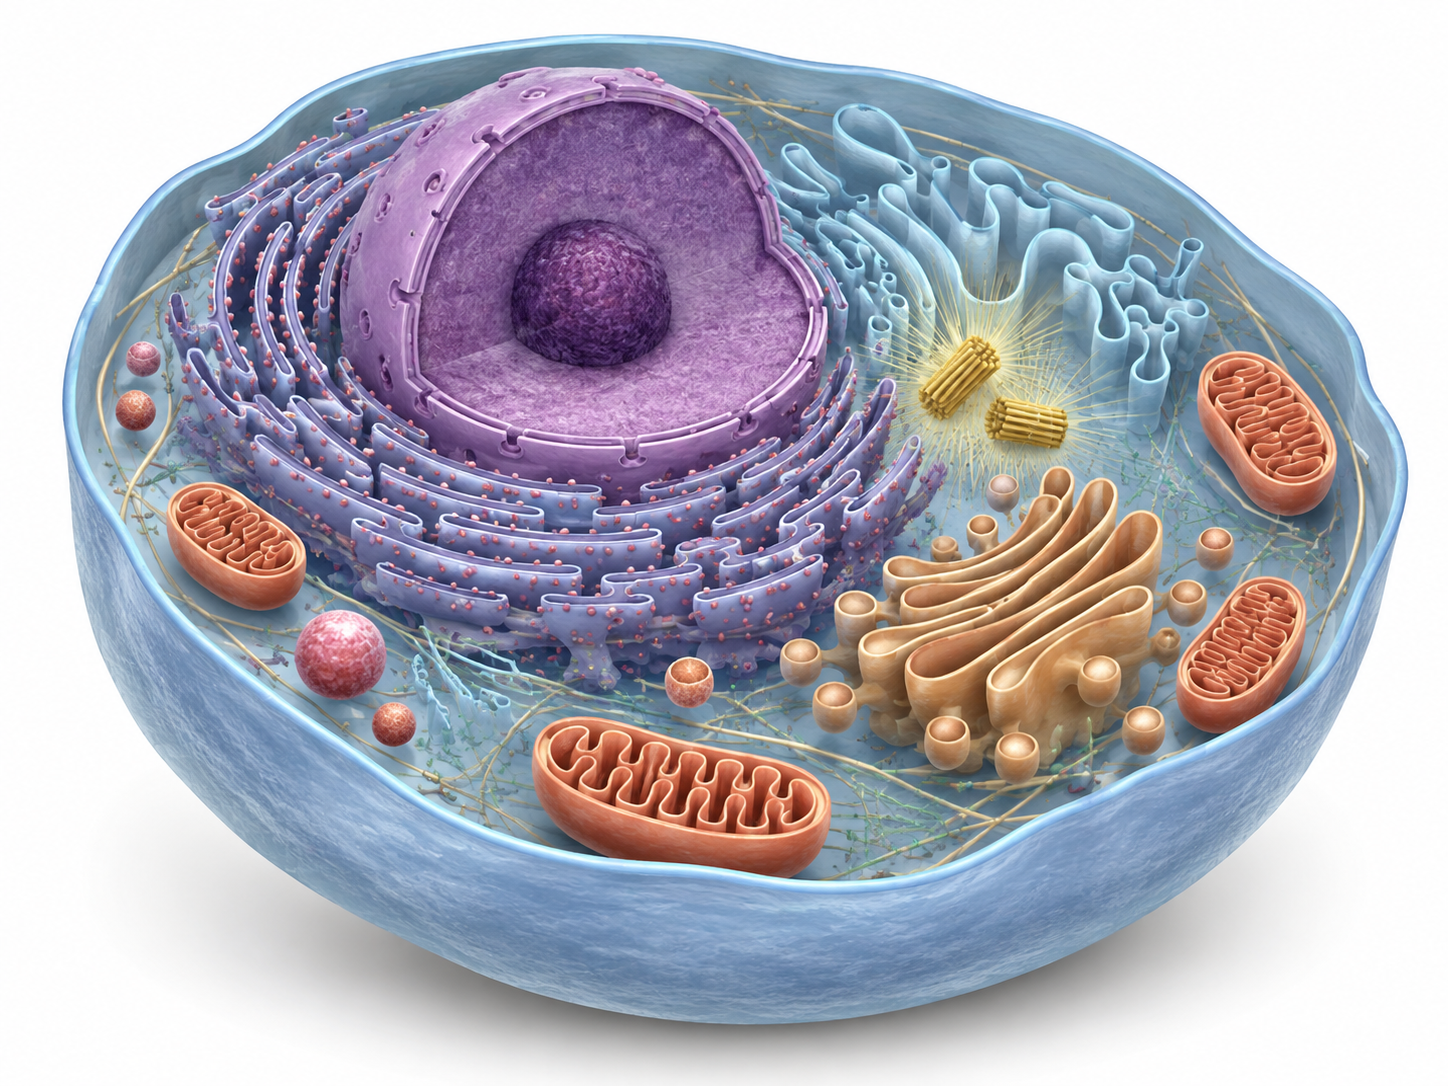
\includegraphics[width=0.6\linewidth]{images/book3/ai/fig-animal-cell-cutaway.png}};
  \begin{scope}[x={(img.south east)}, y={(img.north west)},
      every node/.style={font=\small}]
    \draw[omDef, thick] (0.42,0.72) -- (0.42,1.08) node[above] {núcleo, nucléolo, poros};
    \draw[omDef, thick] (0.30,0.52) -- (-0.03,0.44) node[left, align=right] {retículo endoplasmático\\ rugoso};
    \draw[omDef, thick] (0.23,0.42) -- (-0.03,0.22) node[left] {lisosoma};
    \draw[omDef, thick] (0.07,0.62) -- (-0.03,0.76) node[left] {membrana plasmática};
    \draw[omDef, thick] (0.75,0.80) -- (1.03,0.88) node[right] {RE liso};
    \draw[omDef, thick] (0.69,0.63) -- (1.03,0.62) node[right] {centrosoma};
    \draw[omDef, thick] (0.87,0.42) -- (1.03,0.36) node[right] {mitocondria};
    \draw[omDef, thick] (0.70,0.40) -- (0.80,-0.08) node[below] {aparato de Golgi y vesículas};
    \draw[omDef, thick] (0.47,0.25) -- (0.35,-0.08) node[below] {mitocondria};
  \end{scope}
\end{tikzpicture}

{\small Una \omterm{def:b1:cell-unit-of-life:cell}{célula} animal generalizada, abierta. El \omterm{def:b1:eukaryotic-cell:nucleus}{núcleo} en el centro; a
su alrededor, el \omterm{def:b1:eukaryotic-cell:endomembrane}{retículo endoplasmático rugoso} continuo con la \omterm{def:b1:eukaryotic-cell:nucleus}{envoltura
nuclear}, el retículo liso, la pila del \omterm{def:b1:eukaryotic-cell:endomembrane}{Golgi} y sus vesículas, las
\omterm{def:b1:eukaryotic-cell:mitochondrion}{mitocondrias}, los \omterm{def:b1:eukaryotic-cell:endomembrane}{lisosomas} y el \omterm{def:b1:eukaryotic-cell:cytoskeleton}{centrosoma} del que irradian los
\omterm{def:b1:eukaryotic-cell:cytoskeleton}{microtúbulos}.}
\end{omfigure}

\begin{definition}[El núcleo]\label{def:b1:eukaryotic-cell:nucleus}
El \emph{núcleo}\index{núcleo} contiene los cromosomas en forma de
\emph{cromatina}\index{cromatina}, ADN enrollado sobre proteínas histonas
(\cref{ch:b1:genomes}). Lo delimita la \emph{envoltura
nuclear}\index{envoltura nuclear}, dos membranas de las que la externa es
continua con el \omterm{def:b1:eukaryotic-cell:endomembrane}{retículo endoplasmático}, perforada por \emph{poros
nucleares}\index{poro nuclear} por los que el ARN y las proteínas pasan en
ambos sentidos de forma controlada. El \emph{nucléolo}\index{nucléolo} es la
región donde se fabrica el ARN ribosómico y se ensamblan los ribosomas. El
núcleo separa la transcripción (dentro) de la traducción (fuera), una
separación que los procariotas no tienen.
\end{definition}

\begin{proposition}[Los compartimentos de una célula hepática]\label{prop:b1:eukaryotic-cell:budget}
En un hepatocito de \qty{5000}{\micro m^3}, el \omterm{def:b1:eukaryotic-cell:organelle}{citosol} ocupa
aproximadamente la mitad del volumen, las \omterm{def:b1:eukaryotic-cell:mitochondrion}{mitocondrias} la quinta parte, el
\omterm{def:b1:eukaryotic-cell:endomembrane}{retículo endoplasmático} la sexta, el \omterm{def:b1:eukaryotic-cell:nucleus}{núcleo} la dieciseisava, y el \omterm{def:b1:eukaryotic-cell:endomembrane}{Golgi}, los
\omterm{def:b1:eukaryotic-cell:endomembrane}{lisosomas} y los \omterm{def:b1:eukaryotic-cell:peroxisome}{peroxisomas} unos pocos por ciento entre todos. Las membranas
cuentan otra historia: de los \qty{110000}{\micro m^2} de membrana de la
\omterm{def:b1:cell-unit-of-life:cell}{célula}, la mitad es \omterm{def:b1:eukaryotic-cell:endomembrane}{retículo endoplasmático}, un tercio es la membrana
interna de las \omterm{def:b1:eukaryotic-cell:mitochondrion}{mitocondrias} y solo el \qty{2}{\%} es la membrana plasmática.
Casi toda la membrana de una \omterm{def:b1:cell-unit-of-life:cell}{célula} está dentro de ella.
\end{proposition}

\begin{omfigure}
\begin{tikzpicture}
\begin{axis}[
  xbar, bar width=8pt,
  width=0.72\linewidth, height=6.4cm,
  axis x line=bottom, axis y line=left,
  xmin=0, xmax=45, xlabel={proporción de la membrana total de la célula (\%)},
  xlabel style={font=\small, at={(axis description cs:0.5,-0.13)}, anchor=north},
  symbolic y coords={envoltura nuclear, membrana plasmática, lisosomas y peroxisomas, aparato de Golgi, membrana mitocondrial externa, RE liso, membrana mitocondrial interna, RE rugoso},
  ytick=data, tick label style={font=\small},
  enlarge y limits=0.08, xtick={0,10,20,30,40},
  nodes near coords, nodes near coords style={font=\scriptsize, anchor=west},
]
\addplot[fill=omDef!45, draw=omDef] coordinates
  {(0.2,envoltura nuclear) (2,membrana plasmática) (1.5,lisosomas y peroxisomas) (7,aparato de Golgi) (7,membrana mitocondrial externa) (16,RE liso) (32,membrana mitocondrial interna) (35,RE rugoso)};
\end{axis}
\end{tikzpicture}

{\small Dónde está la membrana de una \omterm{def:b1:cell-unit-of-life:cell}{célula} hepática. La membrana
plasmática, la única visible desde fuera, es el dos por ciento del total; el
retículo y la membrana mitocondrial interna, plegadas dentro, son cuatro
quintas partes.}
\end{omfigure}

\section{El sistema endomembranoso}

\begin{definition}[Retículo endoplasmático, aparato de Golgi, lisosoma]\label{def:b1:eukaryotic-cell:endomembrane}
El \emph{retículo endoplasmático}\index{retículo endoplasmático} (RE) es una
red de láminas y tubos de membrana que encierra un espacio continuo, la luz,
y que se continúa con la \omterm{def:b1:eukaryotic-cell:nucleus}{envoltura nuclear}. Su parte
\emph{rugosa}\index{retículo endoplasmático rugoso} está tachonada de
ribosomas que inyectan las proteínas que fabrican en la luz o en la
membrana; su parte \emph{lisa}\index{retículo endoplasmático liso} fabrica
lípidos, almacena calcio y destoxifica. El \emph{aparato de
Golgi}\index{aparato de Golgi} es una pila de sáculos aplanados (cisternas),
con una cara \emph{cis} de recepción cercana al RE y una cara \emph{trans}
de expedición, en la que las proteínas procedentes del RE se modifican (se
recortan y se añaden azúcares), se clasifican y se empaquetan en vesículas
con destino. Los \emph{lisosomas}\index{lisosoma} son vesículas ácidas (pH
$\approx 5$) llenas de enzimas hidrolíticas que digieren material traído de
fuera u \omterm{def:b1:cell-unit-of-life:prokeuk}{orgánulos} gastados. Junto con las vesículas que se desplazan entre
ellos y la membrana plasmática, todo esto forma el \emph{sistema
endomembranoso}\index{sistema endomembranoso}: un conjunto conectado de
compartimentos cuyas luces son, topológicamente, el exterior de la \omterm{def:b1:cell-unit-of-life:cell}{célula}.
\end{definition}

\begin{proposition}[La vía secretora]\label{prop:b1:eukaryotic-cell:secretory}
\index{vía secretora}
Una proteína destinada a la secreción, a la membrana plasmática o a un
\omterm{def:b1:eukaryotic-cell:endomembrane}{lisosoma} la sintetizan ribosomas unidos al RE rugoso, entra en la luz del RE
a medida que se fabrica, se pliega allí, viaja en vesículas hasta la cara
cis del \omterm{def:b1:eukaryotic-cell:endomembrane}{Golgi}, cruza la pila mientras se modifica y abandona la cara trans
en una vesícula dirigida a su destino: un gránulo de secreción que se
fusiona con la membrana plasmática ante una señal (\emph{exocitosis
regulada}\index{exocitosis}), una vesícula que se fusiona de forma continua
(exocitosis \emph{constitutiva}, que además aporta membrana nueva) o un
\omterm{def:b1:eukaryotic-cell:endomembrane}{lisosoma}. Las proteínas citosólicas y nucleares se fabrican en ribosomas
libres y nunca entran en el sistema. Lo que decide es una \emph{secuencia
señal}\index{secuencia señal} al comienzo de la proteína
(\cref{ch:b1:gene-expression}).
\end{proposition}
\begin{proof}[Evidencia]
Palade (década de 1960) alimentó rodajas de páncreas de cobaya con
aminoácidos radiactivos durante tres minutos (el \emph{pulso}) y después con
aminoácidos sin marcar (la \emph{caza}), y localizó la radiactividad por
autorradiografía de micrografías electrónicas a distintos intervalos. A los
\qty{3}{min} los granos de plata se situaban sobre el RE rugoso; a los
\qty{20}{min}, sobre el \omterm{def:b1:eukaryotic-cell:endomembrane}{Golgi}; a los \qty{40}{min}, sobre \omterm{def:b1:eukaryotic-cell:plantcell}{vacuolas} de
condensación y gránulos nuevos; a las \qty{2}{h}, en la luz del conducto. El
\omterm{def:b1:cell-unit-of-life:fractionation}{fraccionamiento celular} dio la misma secuencia por vía química. Blobel
(década de 1970) mostró que las proteínas de secreción fabricadas en un tubo
de ensayo sin membranas son veinte residuos más largas que la forma
secretada y no quedan protegidas de una proteasa añadida, mientras que si se
fabrican en presencia de membranas del RE se recortan y quedan protegidas:
los residuos de más son la señal que dirige la cadena naciente hacia el RE.
\end{proof}

\begin{omfigure}
\begin{tikzpicture}
\begin{axis}[
  width=0.9\linewidth, height=6.2cm,
  axis x line=bottom, axis y line=left,
  xmin=0, xmax=130, ymin=0, ymax=105,
  xlabel={tiempo tras el pulso (min)}, ylabel={proporción del marcaje (\%)},
  xlabel style={font=\small, at={(axis description cs:0.5,-0.12)}, anchor=north},
  ylabel style={font=\small},
  tick label style={font=\small}, xtick={0,20,40,60,80,100,120}, ytick={0,25,50,75,100},
  legend style={font=\small, at={(0.5,-0.24)}, anchor=north, draw=none, legend columns=2, /tikz/every even column/.append style={column sep=0.4cm}},
  clip=false,
]
\addplot[very thick, omDef, smooth] coordinates {(3,88) (7,55) (15,25) (30,8) (60,2) (120,0)};
\addlegendentry{RE rugoso}
\addplot[very thick, omProp, smooth] coordinates {(3,8) (7,35) (15,55) (30,35) (60,10) (120,2)};
\addlegendentry{Golgi y vacuolas de condensación}
\addplot[very thick, omThm, smooth] coordinates {(3,0) (7,3) (15,12) (30,45) (60,70) (90,55) (120,30)};
\addlegendentry{gránulos de secreción}
\addplot[very thick, omExo, smooth] coordinates {(3,0) (7,0) (15,0) (30,2) (60,12) (90,35) (120,65)};
\addlegendentry{secretado al conducto}
\end{axis}
\end{tikzpicture}

{\small El pulso y caza de Palade en el páncreas: dónde están las proteínas
marcadas en función del tiempo. Pasan del RE al \omterm{def:b1:eukaryotic-cell:endomembrane}{Golgi} en un cuarto de hora,
llegan a los gránulos en menos de una hora y salen de la \omterm{def:b1:cell-unit-of-life:cell}{célula} a lo largo
de las dos siguientes.}
\end{omfigure}

\begin{omfigure}
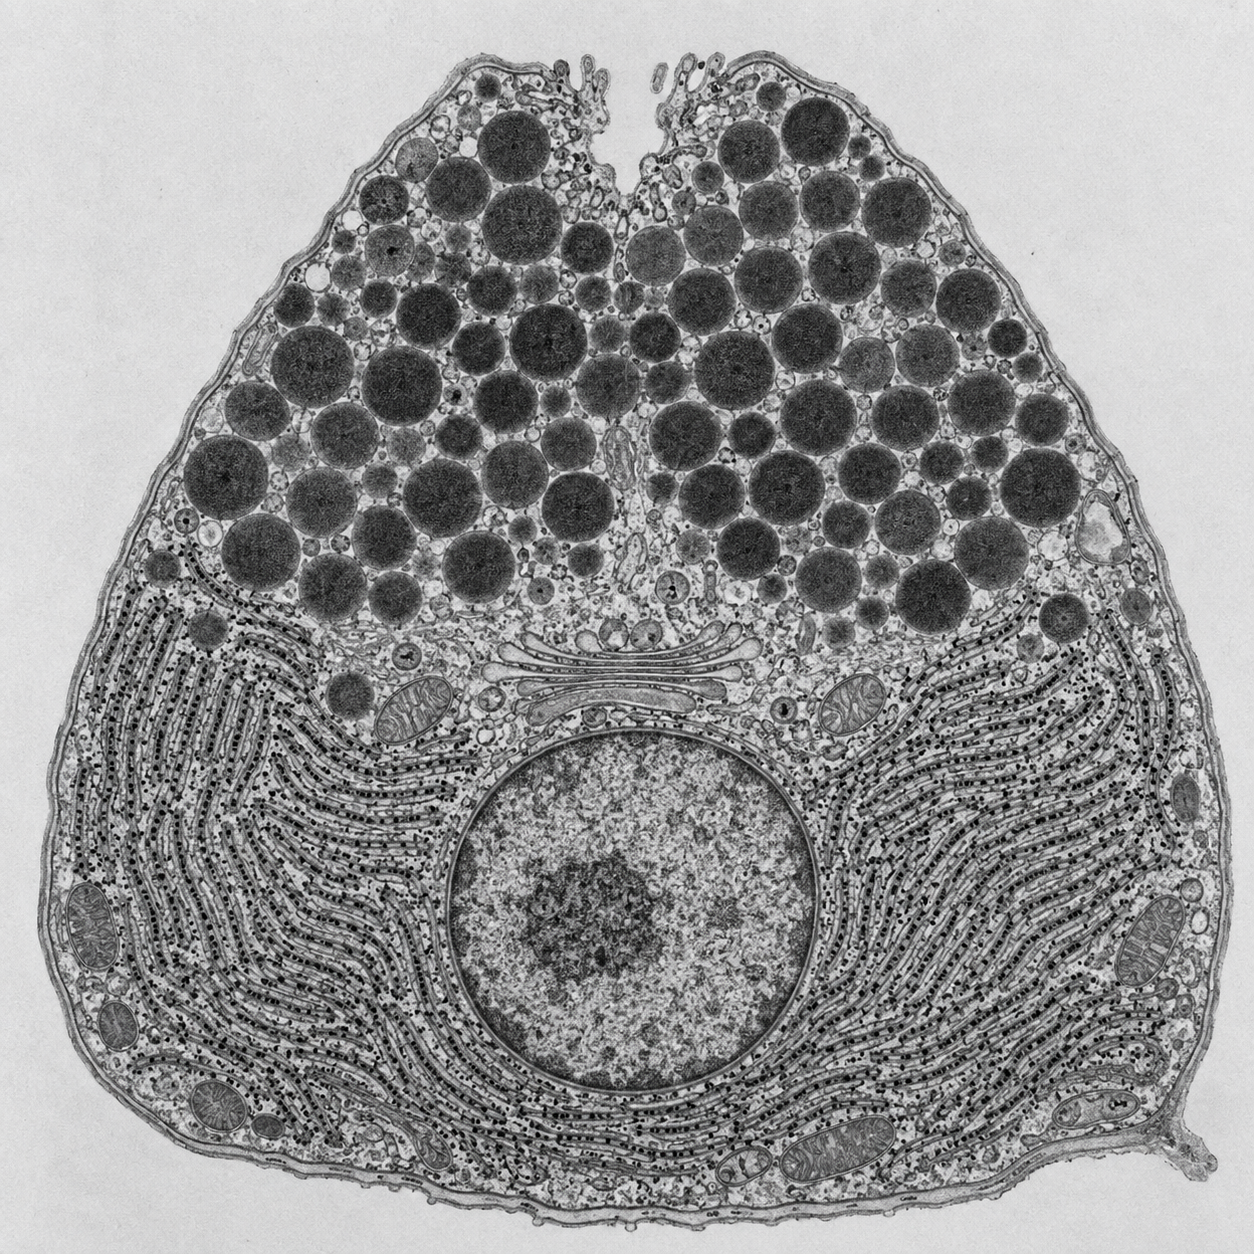
\includegraphics[width=0.44\linewidth]{images/book3/ai/b3-06-acinar-cell-tem.png}

{\small Una \omterm{def:b1:cell-unit-of-life:cell}{célula} acinar pancreática al \omterm{prop:b1:cell-unit-of-life:microscopes}{microscopio electrónico} de
transmisión: RE rugoso apretado en pilas paralelas alrededor del \omterm{def:b1:eukaryotic-cell:nucleus}{núcleo}, en
la base; el \omterm{def:b1:eukaryotic-cell:endomembrane}{Golgi} por encima; y los densos gránulos de secreción
amontonados hacia el ápice y el conducto.}
\end{omfigure}

\begin{method}[Seguir una molécula por la célula]\label{met:b1:eukaryotic-cell:pulsechase}
\begin{enumerate}
  \item Márquese una cohorte breve: expóngase las \omterm{def:b1:cell-unit-of-life:cell}{células} a un precursor
        radiactivo o fluorescente durante unos minutos (el pulso) y
        sustitúyase después por un exceso de precursor sin marcar (la
        caza), de modo que solo las moléculas fabricadas durante el pulso
        lleven el marcaje.
  \item Tómense muestras a intervalos, fíjense y localícese el marcaje: por
        autorradiografía de secciones, por microscopía de fluorescencia o
        por fraccionamiento y recuento.
  \item El compartimento cuyo marcaje culmina primero está aguas arriba; la
        secuencia de máximos es la ruta; los intervalos son los tiempos de
        tránsito.
  \item Bloquéese una etapa (frío, un inhibidor de la energía, un mutante) y
        obsérvese dónde se acumula el marcaje: en el compartimento anterior
        al bloqueo.
\end{enumerate}
\end{method}

\begin{definition}[Endocitosis]\label{def:b1:eukaryotic-cell:endocytosis}
La \emph{endocitosis}\index{endocitosis} hace entrar material: la membrana
plasmática se invagina a su alrededor y estrangula una vesícula, que por lo
general se fusiona con un \omterm{def:b1:eukaryotic-cell:endomembrane}{lisosoma}. La \emph{fagocitosis} engulle partículas
(una bacteria, una \omterm{def:b1:cell-unit-of-life:cell}{célula} muerta); la \emph{pinocitosis} capta gotitas de
líquido; la \emph{endocitosis mediada por receptor} concentra una molécula
concreta (partículas transportadoras de colesterol, transferrina
transportadora de hierro) sobre receptores situados en fositas revestidas
antes de introducirla. La exocitosis añade membrana a la superficie celular
y la endocitosis la retira; en una \omterm{def:b1:cell-unit-of-life:cell}{célula} secretora ambas se compensan, de
modo que la superficie permanece constante mientras áreas enteras de
membrana la recorren cada hora.
\end{definition}

\section{Mitocondrias y plastos}

\begin{definition}[Mitocondria]\label{def:b1:eukaryotic-cell:mitochondrion}
Una \emph{mitocondria}\index{mitocondria} es un \omterm{def:b1:eukaryotic-cell:organelle}{orgánulo} de
\qtyrange{0.5}{1}{\micro m} de ancho y unos micrómetros de largo,
delimitado por dos membranas: una membrana externa lisa, permeable a las
moléculas pequeñas, y una membrana interna plegada en
\emph{crestas}\index{cresta}, impermeable a los iones, que alberga la cadena
respiratoria y la ATP sintasa (\cref{ch:b1:respiration-fermentation}).
Dentro está la \emph{matriz}\index{matriz mitocondrial}, que contiene las
enzimas del ciclo de Krebs, ribosomas de tipo bacteriano y varias copias de
un pequeño ADN circular. Las mitocondrias se dividen por fisión, se
desplazan a lo largo del \omterm{def:b1:eukaryotic-cell:cytoskeleton}{citoesqueleto} y son de unos cientos a unos miles
por \omterm{def:b1:cell-unit-of-life:cell}{célula}.
\end{definition}

\begin{definition}[Plastos]\label{def:b1:eukaryotic-cell:plastid}
Los \emph{plastos}\index{plasto} son los \omterm{def:b1:cell-unit-of-life:prokeuk}{orgánulos} de doble membrana de las
\omterm{def:b1:cell-unit-of-life:cell}{células} vegetales: los \emph{cloroplastos}\index{cloroplasto}, en los que un
tercer sistema de membranas, los \emph{tilacoides}\index{tilacoide},
apilados en granas y bañados por el \emph{estroma}\index{estroma}, lleva a
cabo la fotosíntesis (\cref{ch:b1:photosynthesis}); los amiloplastos, que
almacenan almidón; los cromoplastos, que contienen los pigmentos de frutos y
pétalos. Todos derivan de proplastos y, como las \omterm{def:b1:eukaryotic-cell:mitochondrion}{mitocondrias}, contienen su
propio ADN circular y ribosomas de tipo bacteriano, y se dividen por
fisión.
\end{definition}

\begin{omfigure}
\begin{minipage}[b]{0.48\linewidth}\centering
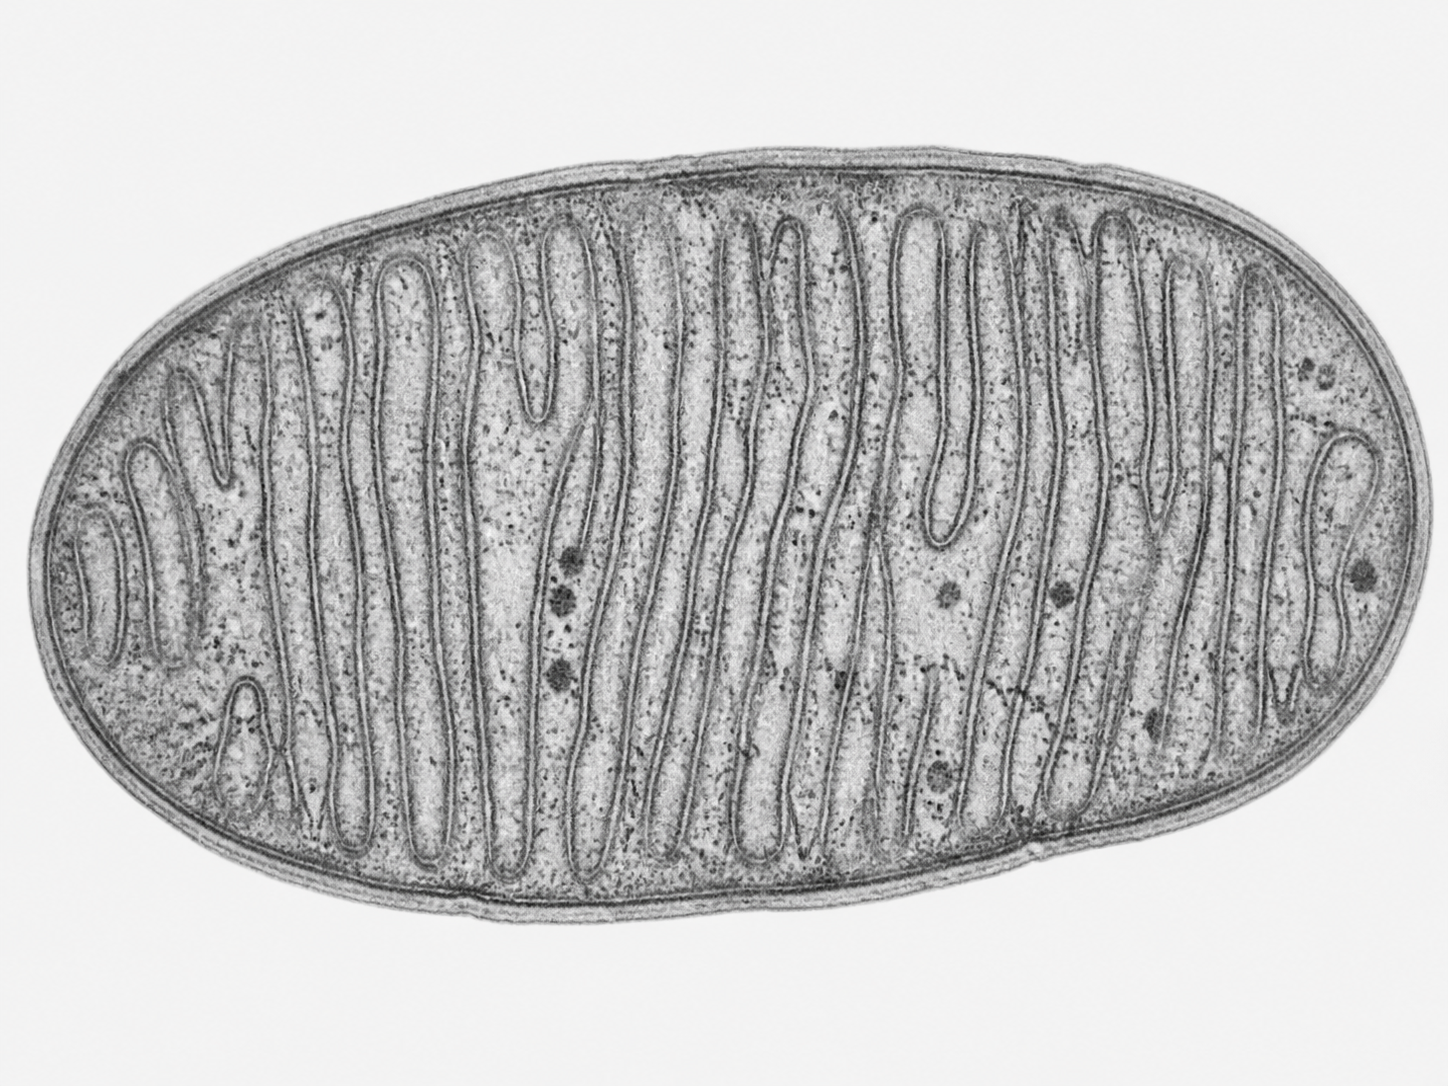
\includegraphics[width=0.96\linewidth]{images/book2/ai/g12-resp-mitochondrion-tem.png}
\end{minipage}\hfill
\begin{minipage}[b]{0.48\linewidth}\centering
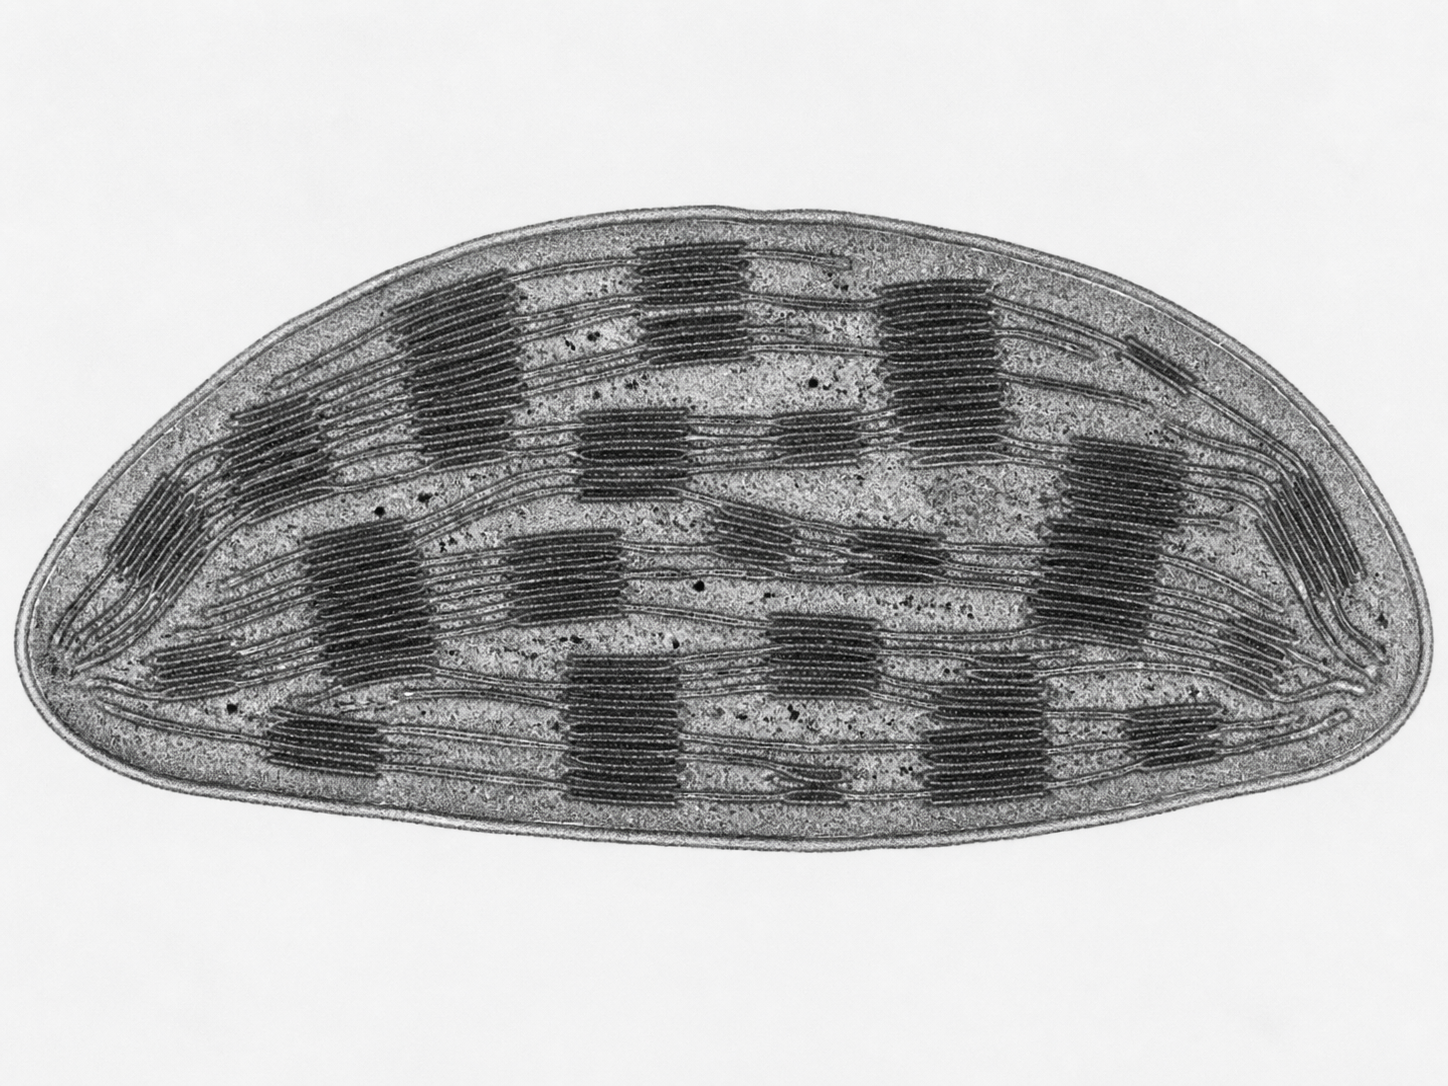
\includegraphics[width=0.96\linewidth]{images/book2/ai/g12-photo-chloroplast-tem.png}
\end{minipage}

{\small Una \omterm{def:b1:eukaryotic-cell:mitochondrion}{mitocondria} (izquierda) y un \omterm{def:b1:eukaryotic-cell:plastid}{cloroplasto} (derecha) en sección al
\omterm{prop:b1:cell-unit-of-life:microscopes}{microscopio electrónico}. Dos membranas de envoltura cada uno; dentro, la
membrana interna plegada de la \omterm{def:b1:eukaryotic-cell:mitochondrion}{mitocondria} y los \omterm{def:b1:eukaryotic-cell:plastid}{tilacoides} apilados del
\omterm{def:b1:eukaryotic-cell:plastid}{cloroplasto}: las membranas sobre las que se transduce la energía.}
\end{omfigure}

\begin{proposition}[Origen endosimbiótico]\label{prop:b1:eukaryotic-cell:endosymbiosis}
\index{endosimbiosis}
Las \omterm{def:b1:eukaryotic-cell:mitochondrion}{mitocondrias} y los \omterm{def:b1:eukaryotic-cell:plastid}{plastos} descienden de bacterias de vida libre
engullidas por una \omterm{def:b1:cell-unit-of-life:prokeuk}{célula eucariota} ancestral y conservadas como simbiontes:
las \omterm{def:b1:eukaryotic-cell:mitochondrion}{mitocondrias}, de una bacteria aerobia; los \omterm{def:b1:eukaryotic-cell:plastid}{plastos}, de una cianobacteria.
\end{proposition}
\begin{proof}[Evidencia]
Ambos \omterm{def:b1:cell-unit-of-life:prokeuk}{orgánulos} tienen dos membranas, la interna de composición bacteriana y
la externa parecida a la del hospedador; un cromosoma circular sin histonas;
ribosomas del tamaño bacteriano y con su misma sensibilidad a los
antibióticos; un código genético con variantes bacterianas; división por
fisión binaria independiente de la de la \omterm{def:b1:cell-unit-of-life:cell}{célula}; y sus genes, al
secuenciarlos, se agrupan con los de linajes bacterianos concretos
(alfaproteobacterias, cianobacterias) y no con los genes nucleares de la
\omterm{def:b1:cell-unit-of-life:cell}{célula} que los aloja. La mayoría de sus genes originales se han trasladado
desde entonces al \omterm{def:b1:eukaryotic-cell:nucleus}{núcleo}, y los \omterm{def:b1:cell-unit-of-life:prokeuk}{orgánulos} ya no pueden vivir solos.
\end{proof}

\begin{definition}[Peroxisoma]\label{def:b1:eukaryotic-cell:peroxisome}
Un \emph{peroxisoma}\index{peroxisoma} es un \omterm{def:b1:eukaryotic-cell:organelle}{orgánulo} pequeño de una sola
membrana que contiene enzimas oxidativas que transfieren hidrógeno desde
distintos sustratos (ácidos grasos, alcohol) al oxígeno, con lo que producen
peróxido de hidrógeno, y catalasa, que destruye el peróxido en el acto.
Confina una química peligrosa.
\end{definition}

\section{El citoesqueleto}

\begin{definition}[Citoesqueleto]\label{def:b1:eukaryotic-cell:cytoskeleton}
El \emph{citoesqueleto}\index{citoesqueleto} es una red de filamentos
proteicos que da a la \omterm{def:b1:cell-unit-of-life:cell}{célula} su forma, ancla sus \omterm{def:b1:cell-unit-of-life:prokeuk}{orgánulos} y los mueve, a
ellos y a la propia \omterm{def:b1:cell-unit-of-life:cell}{célula}. Hay tres clases: los
\emph{microfilamentos}\index{microfilamento} de actina (\qty{7}{nm}, dos
hebras trenzadas de subunidades globulares), concentrados bajo la membrana
plasmática y responsables de la forma celular, la reptación, el anillo
contráctil de la división y la contracción muscular junto con la miosina;
los \emph{microtúbulos}\index{microtúbulo} (tubos huecos de \qty{25}{nm} de
tubulina), que irradian del \emph{centrosoma}\index{centrosoma}, vías por
las que las proteínas motoras (la cinesina hacia fuera, la dineína hacia
dentro) transportan vesículas y \omterm{def:b1:cell-unit-of-life:prokeuk}{orgánulos}, el huso de la división y el eje
de cilios y flagelos; y los \emph{filamentos intermedios}\index{filamento intermedio} (\qty{10}{nm}, en forma de cuerda, de queratinas y proteínas
afines), las fibras mecánicamente resistentes que rigidizan las \omterm{def:b1:cell-unit-of-life:cell}{células} y se
anclan en los desmosomas. Los microfilamentos y los microtúbulos se ensamblan
y se desensamblan sin cesar a partir de sus reservas de subunidades.
\end{definition}

\begin{omfigure}
\begin{tikzpicture}[font=\footnotesize, line cap=round]
  % actin: two twisted strands of beads
  \foreach \i in {0,...,15} {
    \pgfmathsetmacro{\y}{0.13*sin(\i*45)}
    \fill[omThm!70] (0.35*\i,1.6+\y) circle (0.11);
    \fill[omThm!45] (0.35*\i+0.17,1.6-\y) circle (0.11);
  }
  \node[anchor=west, align=left] at (6.0,1.6) {\textbf{microfilamento} (actina), \qty{7}{nm}\\ forma, reptación, anillo de división, músculo};
  % intermediate filament: rope of coiled strands
  \foreach \k in {0,1,2,3} {
    \draw[omProp, thick] plot[domain=0:5.3, samples=60] (\x, {0.55+0.09*sin(180*\x+90*\k)});
  }
  \node[anchor=west, align=left] at (6.0,0.55) {\textbf{filamento intermedio}, \qty{10}{nm}\\ en forma de cuerda, resistencia mecánica};
  % microtubule: hollow tube of protofilaments
  \draw[thick, omDef!70!black, fill=omDef!15] (0,-0.9) rectangle (5.3,-0.2);
  \foreach \i in {0,...,25} { \foreach \j in {0,1,2,3} {
    \fill[omDef!60] (0.1+0.2*\i, -0.83+0.19*\j) circle (0.075);
  } }
  \draw[thick, omDef!70!black, fill=omDef!10] (5.3,-0.55) ellipse (0.18 and 0.35);
  \draw[thick, omDef!70!black, fill=white] (5.3,-0.55) ellipse (0.10 and 0.24);
  \node[anchor=west, align=left] at (6.0,-0.55) {\textbf{microtúbulo} (tubulina), hueco, \qty{25}{nm}\\ vías para los motores, huso, cilios};
\end{tikzpicture}

{\small Los tres filamentos del \omterm{def:b1:eukaryotic-cell:cytoskeleton}{citoesqueleto}, dibujados a la misma escala.
La actina y la tubulina polimerizan de forma reversible a partir de
subunidades globulares; los \omterm{def:b1:eukaryotic-cell:cytoskeleton}{filamentos intermedios} son cuerdas estables.}
\end{omfigure}

\begin{example}[Mover una vesícula]\label{ex:b1:eukaryotic-cell:transport}
Una vesícula de secreción que sale del \omterm{def:b1:eukaryotic-cell:endomembrane}{Golgi} la recoge la cinesina, un motor
que camina por un \omterm{def:b1:eukaryotic-cell:cytoskeleton}{microtúbulo} hacia la periferia celular a unos
\qty{1}{\micro m/s} y gasta un ATP por cada paso de \qty{8}{nm}; en una
\omterm{def:b1:body-plans-tissues:nervous}{neurona} ese mismo motor lleva vesículas a lo largo de un axón de un metro,
un viaje de diez días. Cerca de la superficie, la vesícula pasa al córtex de
actina y a la miosina para el último micrómetro. La difusión tardaría cerca
de un minuto en llevar una vesícula de \qty{100}{nm} a través de una \omterm{def:b1:cell-unit-of-life:cell}{célula}
de \qty{20}{\micro m}, y años en recorrer un metro: los \omterm{def:b1:cell-unit-of-life:prokeuk}{orgánulos} se
transportan, no se dejan vagar.
\end{example}

\section{Células vegetales y animales}

\begin{definition}[Pared celular, vacuola, plasmodesmos]\label{def:b1:eukaryotic-cell:plantcell}
Una \omterm{def:b1:cell-unit-of-life:cell}{célula} vegetal añade tres estructuras al plan común. La \emph{pared
celular}\index{pared celular}, por fuera de la membrana plasmática, es un
compuesto de microfibrillas de celulosa en una matriz de otros polisacáridos
(\cref{ch:b1:carbohydrates}); fija la forma de la \omterm{def:b1:cell-unit-of-life:cell}{célula}, resiste la presión
interior y cementa entre sí las \omterm{def:b1:cell-unit-of-life:cell}{células} vecinas mediante una lámina media
compartida. La \emph{vacuola}\index{vacuola}, un compartimento de una sola
membrana que ocupa hasta el \qty{90}{\%} del volumen de la \omterm{def:b1:cell-unit-of-life:cell}{célula}, almacena
agua, iones, azúcares, pigmentos y desechos; su presión osmótica empuja la
membrana contra la pared, y esa \emph{turgencia}\index{turgencia} es lo que
mantiene erguida una \omterm{def:b1:flowering-plant-organization:organs}{hoja}. Los \emph{plasmodesmos}\index{plasmodesmo} son
canales que atraviesan las paredes, revestidos de membrana plasmática, por
los que los \omterm{def:b1:eukaryotic-cell:organelle}{citosoles} de \omterm{def:b1:cell-unit-of-life:cell}{células} vecinas quedan en continuidad, de modo que
un \omterm{def:b1:body-plans-tissues:tissue}{tejido} vegetal es en parte un solo \omterm{def:b1:cell-unit-of-life:cell}{citoplasma} conectado (el simplasto).
\end{definition}

\begin{omfigure}
\begin{tikzpicture}
  \node[anchor=south west, inner sep=0] (img) at (0,0)
    {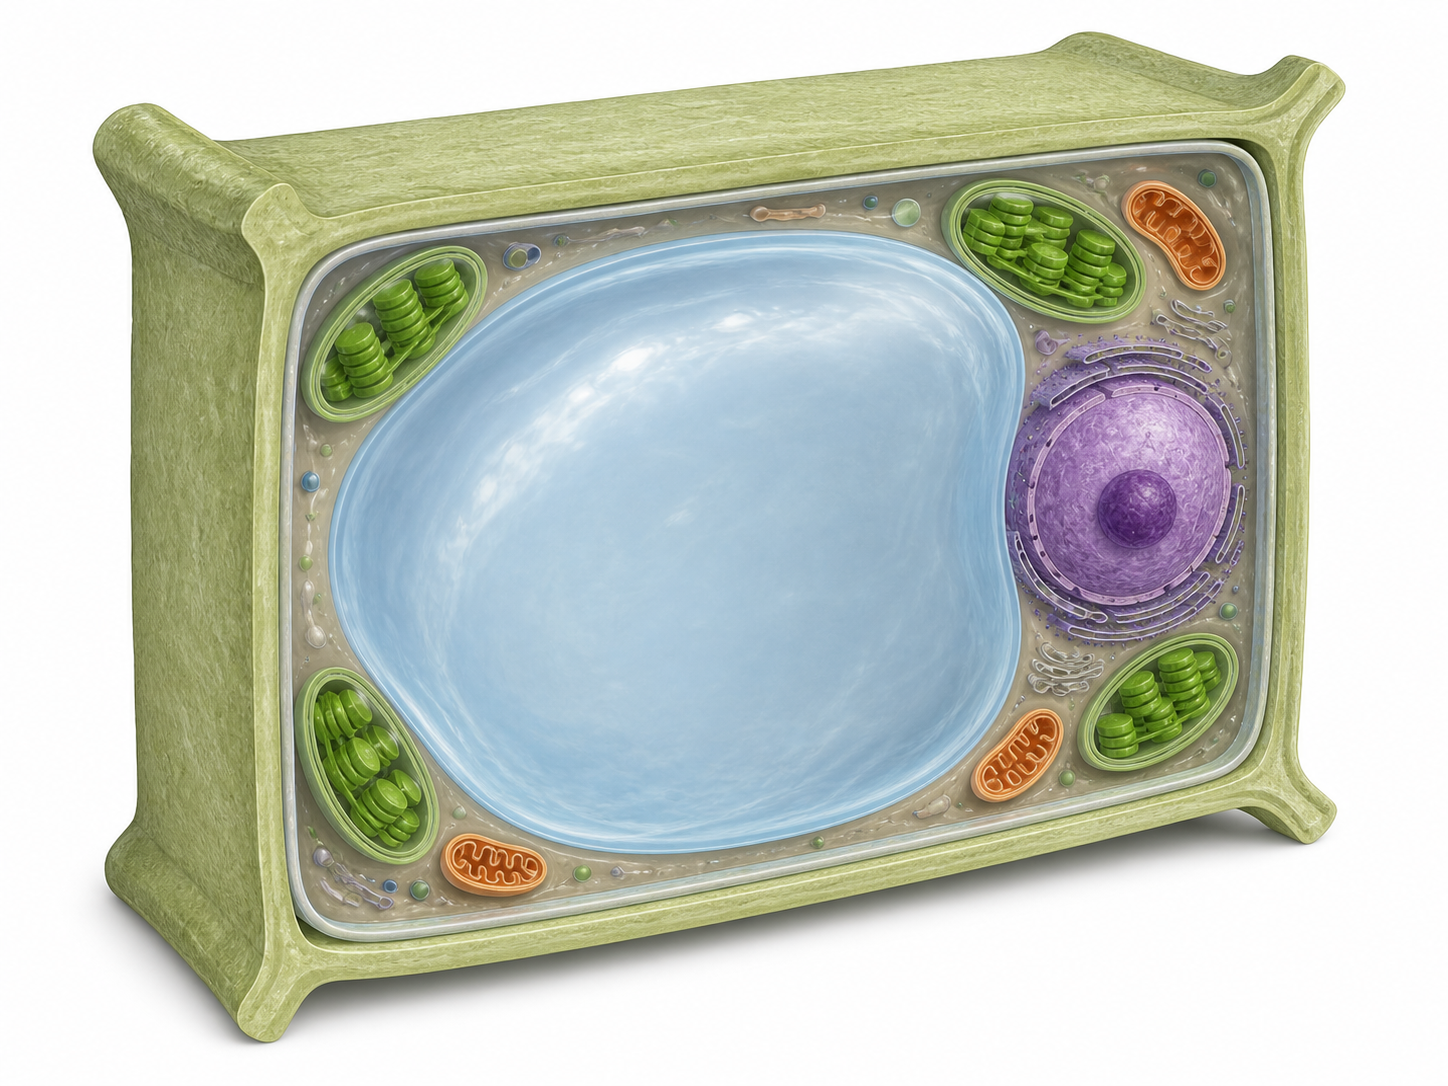
\includegraphics[width=0.52\linewidth]{images/book2/ai/fig-plant-cell-cutaway-v2.png}};
  \begin{scope}[x={(img.south east)}, y={(img.north west)},
      every node/.style={font=\small}]
    \draw[omDef, thick] (0.50,0.50) -- (0.50,1.08) node[above] {vacuola central};
    \draw[omDef, thick] (0.10,0.50) -- (-0.03,0.56) node[left] {pared celular};
    \draw[omDef, thick] (0.25,0.73) -- (-0.03,0.84) node[left] {cloroplasto};
    \draw[omDef, thick] (0.35,0.17) -- (-0.03,0.12) node[left] {mitocondria};
    \draw[omDef, thick] (0.76,0.47) -- (1.03,0.60) node[right] {núcleo};
    \draw[omDef, thick] (0.60,0.13) -- (1.03,0.16) node[right] {citoplasma delgado};
  \end{scope}
\end{tikzpicture}

{\small Una \omterm{def:b1:cell-unit-of-life:cell}{célula} vegetal: la pared por fuera de la membrana, la \omterm{def:b1:eukaryotic-cell:plantcell}{vacuola}
ocupando casi todo el volumen, y \omterm{def:b1:eukaryotic-cell:plastid}{cloroplastos} y \omterm{def:b1:eukaryotic-cell:mitochondrion}{mitocondrias} en la delgada
capa de \omterm{def:b1:cell-unit-of-life:cell}{citoplasma} que queda entre ambas.}
\end{omfigure}

\begin{proposition}[Célula vegetal y célula animal comparadas]\label{prop:b1:eukaryotic-cell:compare}
Ambas tienen \omterm{def:b1:eukaryotic-cell:nucleus}{núcleo}, RE, \omterm{def:b1:eukaryotic-cell:endomembrane}{Golgi}, \omterm{def:b1:eukaryotic-cell:mitochondrion}{mitocondrias}, \omterm{def:b1:eukaryotic-cell:peroxisome}{peroxisomas}, ribosomas y
\omterm{def:b1:eukaryotic-cell:cytoskeleton}{citoesqueleto}. La \omterm{def:b1:cell-unit-of-life:cell}{célula} vegetal tiene una pared de celulosa, una \omterm{def:b1:eukaryotic-cell:plantcell}{vacuola}
grande, \omterm{def:b1:eukaryotic-cell:plastid}{plastos} y \omterm{def:b1:eukaryotic-cell:plantcell}{plasmodesmos}, y carece de centriolos y de \omterm{def:b1:eukaryotic-cell:endomembrane}{lisosomas} (la
\omterm{def:b1:eukaryotic-cell:plantcell}{vacuola} digiere); no repta ni engulle, y se divide construyendo una pared
nueva por el medio. La \omterm{def:b1:cell-unit-of-life:cell}{célula} animal no tiene pared (y por eso puede cambiar
de forma, reptar y fagocitar), tiene \omterm{def:b1:eukaryotic-cell:endomembrane}{lisosomas} y un \omterm{def:b1:eukaryotic-cell:cytoskeleton}{centrosoma} con
centriolos, y se comunica por uniones en vez de por \omterm{def:b1:eukaryotic-cell:plantcell}{plasmodesmos}; se divide
estrangulándose en dos.
\end{proposition}

\begin{example}[Turgencia]\label{ex:b1:eukaryotic-cell:turgor}
Una \omterm{def:b1:cell-unit-of-life:cell}{célula} foliar cuya \omterm{def:b1:eukaryotic-cell:plantcell}{vacuola} contiene \qty{0.3}{mol/L} de solutos absorbe
agua hasta que la pared devuelve una presión de unos \qty{0.7}{MPa}, siete
atmósferas; la \omterm{def:b1:cell-unit-of-life:cell}{célula} está entonces turgente y la \omterm{def:b1:flowering-plant-organization:organs}{hoja}, firme. Privada de
agua, la \omterm{def:b1:eukaryotic-cell:plantcell}{vacuola} pierde volumen, la presión cae a cero y la \omterm{def:b1:flowering-plant-organization:organs}{hoja} se marchita
--- la pared intacta, la presión desaparecida
(\cref{ch:b1:membranes-transport}). Una \omterm{def:b1:cell-unit-of-life:cell}{célula} animal en la misma
disolución, al no tener pared, simplemente reventaría.
\end{example}

\section{Ejercicios}

\begin{exercise}[$\star$]\label{exo:b1:eukaryotic-cell:1}
Enumérense los \omterm{def:b1:cell-unit-of-life:prokeuk}{orgánulos} delimitados por membrana de una \omterm{def:b1:cell-unit-of-life:cell}{célula} animal y
dese en pocas palabras la función principal de cada uno.
\end{exercise}

\begin{exercise}[$\star$]\label{exo:b1:eukaryotic-cell:2}
Trácese el camino de una enzima digestiva desde su síntesis hasta el
conducto, nombrando cada compartimento y el modo en que la proteína pasa de
uno a otro.
\end{exercise}

\begin{exercise}[$\star$]\label{exo:b1:eukaryotic-cell:3}
A partir de la figura del reparto de membrana, ¿qué fracción de la membrana
de la \omterm{def:b1:cell-unit-of-life:cell}{célula} es mitocondrial (externa más interna)? ¿Por qué la membrana
interna es tanto mayor que la externa?
\end{exercise}

\begin{exercise}[$\star$]\label{exo:b1:eukaryotic-cell:4}
Dense tres estructuras que tenga una \omterm{def:b1:cell-unit-of-life:cell}{célula} vegetal y le falten a una animal,
y dos que tenga la animal y le falten a la vegetal.
\end{exercise}

\begin{exercise}[$\star\star$]\label{exo:b1:eukaryotic-cell:5}
A partir de la figura del pulso y caza, ¿en qué momento culmina el marcaje
en el RE, en el \omterm{def:b1:eukaryotic-cell:endomembrane}{Golgi} y en los gránulos? Estímense el tiempo de tránsito del
RE al gránulo y el tiempo que pasa hasta que se ha secretado la mitad del
marcaje.
\end{exercise}

\begin{exercise}[$\star\star$]\label{exo:b1:eukaryotic-cell:6}
Se trata una \omterm{def:b1:cell-unit-of-life:cell}{célula} con un fármaco que despolimeriza los \omterm{def:b1:eukaryotic-cell:cytoskeleton}{microtúbulos}.
Predíganse los efectos sobre la posición del \omterm{def:b1:eukaryotic-cell:endomembrane}{Golgi}, sobre el tráfico de
vesículas, sobre la división celular y sobre el batido de los cilios.
\end{exercise}

\begin{exercise}[$\star\star$]\label{exo:b1:eukaryotic-cell:7}
Dense cuatro pruebas del origen bacteriano de las \omterm{def:b1:eukaryotic-cell:mitochondrion}{mitocondrias} y explíquese
por qué, pese a ello, una \omterm{def:b1:eukaryotic-cell:mitochondrion}{mitocondria} no puede vivir fuera de una \omterm{def:b1:cell-unit-of-life:cell}{célula}.
\end{exercise}

\begin{exercise}[$\star\star$]\label{exo:b1:eukaryotic-cell:8}
La luz del RE está ``topológicamente fuera de la \omterm{def:b1:cell-unit-of-life:cell}{célula}''. Explíquese la
expresión siguiendo una proteína de membrana cuyas cadenas de azúcares miran
a la luz desde el RE hasta la membrana plasmática: ¿hacia qué lado miran los
azúcares al final?
\end{exercise}

\begin{exercise}[$\star\star$]\label{exo:b1:eukaryotic-cell:9}
Una \omterm{def:b1:cell-unit-of-life:cell}{célula} secretora libera \qty{2000}{} gránulos de \qty{1}{\micro m} de
diámetro al día por una superficie apical de \qty{40}{\micro m^2}.
Calcúlense la membrana añadida por día y cuántas veces debe reciclarse la
superficie apical. ¿Qué implica esto?
\end{exercise}

\begin{exercise}[$\star\star\star$]\label{exo:b1:eukaryotic-cell:10}
En un tubo de ensayo con ribosomas, ARNm de una proteína de secreción y
aminoácidos, el producto es una cadena de \qty{320}{} residuos; al añadir
vesículas del RE, aparece dentro de las vesículas una cadena de \qty{300}{}
residuos que una proteasa añadida después no digiere. Interprétese cada
observación, y dígase qué haría un mutante que careciera de los veinte
primeros residuos.
\end{exercise}

\begin{exercise}[$\star\star\star$]\label{exo:b1:eukaryotic-cell:11}
Las \omterm{def:b1:cell-unit-of-life:cell}{células} de un paciente carecen de una enzima lisosómica que degrada un
lípido; el lípido se acumula en \omterm{def:b1:eukaryotic-cell:endomembrane}{lisosomas} hinchados y las \omterm{def:b1:cell-unit-of-life:cell}{células} mueren.
Explíquese la biología celular, dígase por qué la enfermedad es más grave en
las \omterm{def:b1:cell-unit-of-life:cell}{células} que renuevan más deprisa sus membranas, y propóngase cómo podría
una enzima inyectada en la sangre llegar a los \omterm{def:b1:eukaryotic-cell:endomembrane}{lisosomas}.
\end{exercise}

\begin{exercise}[$\star\star\star$]\label{exo:b1:eukaryotic-cell:12}
``La \omterm{def:b1:cell-unit-of-life:prokeuk}{célula eucariota} es una federación de antiguas bacterias mantenida
unida por un sistema de membranas.'' Discútase en un párrafo, sopesando lo
que la teoría endosimbiótica explica frente a lo que no explica (\omterm{def:b1:eukaryotic-cell:nucleus}{núcleo}, RE,
\omterm{def:b1:eukaryotic-cell:cytoskeleton}{citoesqueleto}).
\end{exercise}

\section{Problema: la célula acinar del páncreas}

\begin{problem}[{Problema de fin de semana --- una célula que secreta cada
día su propia masa de proteína: el reloj de Palade, la membrana que debe
reciclar, la señal que dirige la proteína, hasta llegar al tiempo de
tránsito de una enzima digestiva}]
\label{pb:b1:eukaryotic-cell:1}
Una \omterm{def:b1:cell-unit-of-life:cell}{célula} acinar pancreática es un cubo de \qty{12}{\micro m} de lado, con
su cara apical (\qty{144}{\micro m^2}, sobre el conducto) y su cara basal
sobre la sangre. Un páncreas humano de \qty{80}{g} contiene unos
$\num{8e10}$ \omterm{def:b1:cell-unit-of-life:cell}{células} de este tipo y secreta \qty{10}{g} de proteína
enzimática al día. Un gránulo de secreción es una esfera de \qty{1}{\micro m}
de diámetro que contiene proteína a \qty{200}{mg/mL}. Los ribosomas añaden
\qty{5}{} aminoácidos por segundo; una enzima típica tiene \qty{250}{}
residuos de masa media \qty{110}{g/mol}.

\medskip
\noindent\textbf{Parte I --- El reloj de Palade.}
La figura del pulso y caza del capítulo da la localización del marcaje con
el tiempo.
\begin{enumerate}
  \item ¿Por qué debe ser corto el pulso y contener la caza un gran exceso
        de aminoácido sin marcar?
  \item Léase el momento en que el marcaje culmina en el RE, en el \omterm{def:b1:eukaryotic-cell:endomembrane}{Golgi} y
        en los gránulos.
  \item Estímense el tiempo de tránsito del RE al \omterm{def:b1:eukaryotic-cell:endomembrane}{Golgi} y el del \omterm{def:b1:eukaryotic-cell:endomembrane}{Golgi} al
        gránulo.
  \item ¿Dónde está el marcaje a los \qty{60}{min}, y por qué una parte ha
        salido ya de la \omterm{def:b1:cell-unit-of-life:cell}{célula} mientras la mayor parte sigue en gránulos?
  \item Se hace un segundo experimento a \qty{15}{\celsius}: el marcaje
        permanece en el RE más de una hora. Interprétese.
\end{enumerate}

\medskip
\noindent\textbf{Parte II --- La masa de proteína.}
\begin{enumerate}[resume]
  \item Calcúlese la proteína secretada por \omterm{def:b1:cell-unit-of-life:cell}{célula} y día, en picogramos.
  \item Calcúlense el volumen de un gránulo y la masa de proteína que
        contiene.
  \item Calcúlese el número de gránulos liberados por \omterm{def:b1:cell-unit-of-life:cell}{célula} y día, y por
        minuto.
  \item Calcúlense el volumen de la \omterm{def:b1:cell-unit-of-life:cell}{célula} y, con una densidad de
        \qty{1.05}{g/cm^3}, su masa. ¿Qué fracción de su propia masa
        secreta cada día?
  \item Calcúlese el número de moléculas de enzima de un gránulo (número de
        Avogadro $\num{6.0e23}$).
  \item Calcúlese el tiempo que necesita un ribosoma para fabricar una
        molécula de enzima.
  \item ¿Cuántos ribosomas deben trabajar sin parar para producir la
        cantidad diaria? Compárese con los $\num{4e6}$ ribosomas que
        contiene una \omterm{def:b1:cell-unit-of-life:cell}{célula} así.
\end{enumerate}

\medskip
\noindent\textbf{Parte III --- Membrana.}
\begin{enumerate}[resume]
  \item Calcúlese el área de membrana de un gránulo.
  \item Calcúlese la membrana entregada a la cara apical al día por la
        exocitosis de los gránulos de la pregunta 8.
  \item ¿Cuántas veces al día se añade el área de la cara apical? ¿Qué debe
        hacer la \omterm{def:b1:cell-unit-of-life:cell}{célula} con ella, y mediante qué proceso?
  \item La membrana del gránulo llega del \omterm{def:b1:eukaryotic-cell:endomembrane}{Golgi}, que la recibe del RE. Si
        el RE de la \omterm{def:b1:cell-unit-of-life:cell}{célula} tiene \qty{20000}{\micro m^2} de membrana,
        ¿a cuántos días de membrana de gránulos equivale? ¿Qué dice esto
        sobre el reciclaje dentro del \omterm{def:b1:eukaryotic-cell:endomembrane}{sistema endomembranoso}?
  \item La cara apical lleva \qty{2000}{} microvellosidades de
        \qty{0.1}{\micro m} de diámetro y \qty{1}{\micro m} de longitud.
        ¿En qué factor agrandan la cara de \qty{144}{\micro m^2}?
\end{enumerate}

\medskip
\noindent\textbf{Parte IV --- La dirección escrita en la proteína.}
\begin{enumerate}[resume]
  \item El ARNm de una enzima traducido en un tubo de ensayo sin membranas
        da una cadena \qty{20}{} residuos más larga que la enzima hallada
        en los gránulos. ¿Dónde están los residuos de más y qué son?
  \item En presencia de vesículas del RE, el producto tiene la longitud
        correcta, está dentro de las vesículas y queda protegido de una
        proteasa. Interprétese.
  \item El mismo experimento con el ARNm de una enzima citosólica da un
        producto fuera de las vesículas y sin protección. Conclúyase.
  \item Una mutación elimina los veinte residuos. Predígase dónde acaba la
        enzima y qué le ocurre a la \omterm{def:b1:cell-unit-of-life:cell}{célula}.
  \item Otra enzima aparece en los \omterm{def:b1:eukaryotic-cell:endomembrane}{lisosomas} y no en los gránulos. Lleva la
        misma clase de \omterm{prop:b1:eukaryotic-cell:secretory}{secuencia señal}. ¿En qué punto de la vía debe
        tomarse la segunda decisión, y mediante qué mecanismo, a grandes
        rasgos?
  \item Se trata una \omterm{def:b1:cell-unit-of-life:cell}{célula} con un fármaco que bloquea la síntesis de ATP.
        Predígase dónde se acumula el marcaje de un pulso y caza y por qué
        (dos razones).
  \item Combínense las preguntas 3 y 8: en estado estacionario, ¿cuántos
        gránulos hay ``en tránsito'' entre el RE y el gránulo en cada
        momento?
  \item Resúmase el resultado: el tiempo de tránsito de la síntesis al
        gránulo, el tiempo hasta la secreción, los gránulos liberados por
        minuto y la fracción de su propia masa que secreta la \omterm{def:b1:cell-unit-of-life:cell}{célula} cada
        día.
\end{enumerate}
\end{problem}
